% Options for packages loaded elsewhere
\PassOptionsToPackage{unicode}{hyperref}
\PassOptionsToPackage{hyphens}{url}
%
\documentclass[
  ignorenonframetext,
]{beamer}
\title{CIERRE DIPLOMADO - ENTREGA DE CERTIFICADOS}
\subtitle{Diplomado en Análisis de datos con R para la Acuicultura.}
\author{Dr.~José Gallardo Matus}
\date{29 July 2022}
\institute{Pontificia Universidad Católica de Valparaíso}

\usepackage{pgfpages}
\setbeamertemplate{caption}[numbered]
\setbeamertemplate{caption label separator}{: }
\setbeamercolor{caption name}{fg=normal text.fg}
\beamertemplatenavigationsymbolsempty
% Prevent slide breaks in the middle of a paragraph
\widowpenalties 1 10000
\raggedbottom
\setbeamertemplate{part page}{
  \centering
  \begin{beamercolorbox}[sep=16pt,center]{part title}
    \usebeamerfont{part title}\insertpart\par
  \end{beamercolorbox}
}
\setbeamertemplate{section page}{
  \centering
  \begin{beamercolorbox}[sep=12pt,center]{part title}
    \usebeamerfont{section title}\insertsection\par
  \end{beamercolorbox}
}
\setbeamertemplate{subsection page}{
  \centering
  \begin{beamercolorbox}[sep=8pt,center]{part title}
    \usebeamerfont{subsection title}\insertsubsection\par
  \end{beamercolorbox}
}
\AtBeginPart{
  \frame{\partpage}
}
\AtBeginSection{
  \ifbibliography
  \else
    \frame{\sectionpage}
  \fi
}
\AtBeginSubsection{
  \frame{\subsectionpage}
}
\usepackage{amsmath,amssymb}
\usepackage{lmodern}
\usepackage{iftex}
\ifPDFTeX
  \usepackage[T1]{fontenc}
  \usepackage[utf8]{inputenc}
  \usepackage{textcomp} % provide euro and other symbols
\else % if luatex or xetex
  \usepackage{unicode-math}
  \defaultfontfeatures{Scale=MatchLowercase}
  \defaultfontfeatures[\rmfamily]{Ligatures=TeX,Scale=1}
\fi
\usetheme[]{Malmoe}
\usecolortheme{seahorse}
\usefonttheme{professionalfonts}
% Use upquote if available, for straight quotes in verbatim environments
\IfFileExists{upquote.sty}{\usepackage{upquote}}{}
\IfFileExists{microtype.sty}{% use microtype if available
  \usepackage[]{microtype}
  \UseMicrotypeSet[protrusion]{basicmath} % disable protrusion for tt fonts
}{}
\makeatletter
\@ifundefined{KOMAClassName}{% if non-KOMA class
  \IfFileExists{parskip.sty}{%
    \usepackage{parskip}
  }{% else
    \setlength{\parindent}{0pt}
    \setlength{\parskip}{6pt plus 2pt minus 1pt}}
}{% if KOMA class
  \KOMAoptions{parskip=half}}
\makeatother
\usepackage{xcolor}
\IfFileExists{xurl.sty}{\usepackage{xurl}}{} % add URL line breaks if available
\IfFileExists{bookmark.sty}{\usepackage{bookmark}}{\usepackage{hyperref}}
\hypersetup{
  pdftitle={CIERRE DIPLOMADO - ENTREGA DE CERTIFICADOS},
  pdfauthor={Dr.~José Gallardo Matus},
  hidelinks,
  pdfcreator={LaTeX via pandoc}}
\urlstyle{same} % disable monospaced font for URLs
\newif\ifbibliography
\setlength{\emergencystretch}{3em} % prevent overfull lines
\providecommand{\tightlist}{%
  \setlength{\itemsep}{0pt}\setlength{\parskip}{0pt}}
\setcounter{secnumdepth}{-\maxdimen} % remove section numbering
\newcommand{\columnsbegin}{\begin{columns}}
\newcommand{\columnsend}{\end{columns}}
\ifLuaTeX
  \usepackage{selnolig}  % disable illegal ligatures
\fi

\begin{document}
\frame{\titlepage}

\begin{frame}{PLAN DE LA CEREMONIA DE CIERRE}
\protect\hypertarget{plan-de-la-ceremonia-de-cierre}{}
\begin{itemize}
\item
  Palabras Director del Diplomado.
\item
  Palabras Director del Doctorado.
\item
  Entrega certificados graduados.
\item
  Reconocimiento de excelencia académica.
\item
  Palabras de cierre.
\end{itemize}
\end{frame}

\begin{frame}{PALABRAS DIRECTOR DIPLOMADO}
\protect\hypertarget{palabras-director-diplomado}{}
\textbf{Programa consolidado}\\
1ra y 2da versión: 45 graduados.\\
3ra versión: 22 graduados.\\
Total: 67 graduados.

\textbf{Perfil del graduado}\\
Chile: 70 \%\\
Ecuador: 7 \%\\
México: 7 \%\\
Perú: 7 \%\\
Colombia: 5 \%\\
Venezuela: 1 \%\\
Argentina: 1 \%\\
Hombres: 66 \%\\
Mujeres: 34 \%
\end{frame}

\begin{frame}{EVALUACIÓN DIPLOMADO}
\protect\hypertarget{evaluaciuxf3n-diplomado}{}
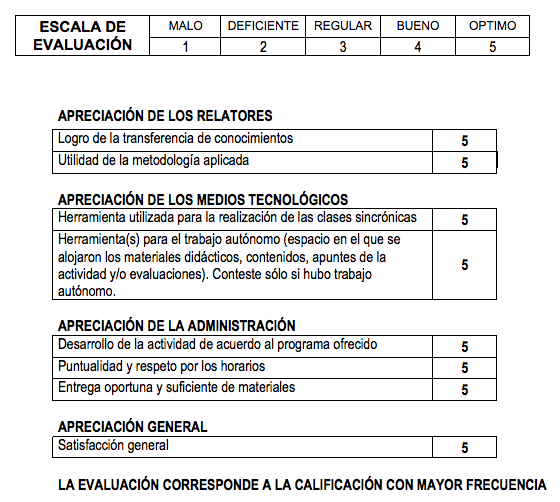
\includegraphics[width=0.6\linewidth]{Evaluacion}
\end{frame}

\begin{frame}{AGRADECIMIENTO AL EQUIPO}
\protect\hypertarget{agradecimiento-al-equipo}{}
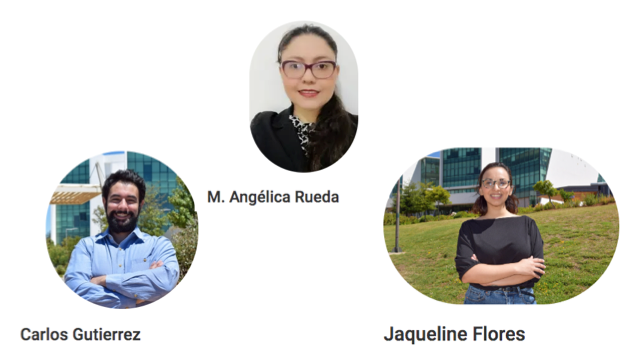
\includegraphics[width=0.8\linewidth]{Equipo}
\end{frame}

\begin{frame}{PALABRAS DIRECTOR DOCTORADO}
\protect\hypertarget{palabras-director-doctorado}{}
\begin{itemize}
\item
  \textbf{Dr.~Felipe Hurtado}\\
  Jefe de Vinculación con el Medio.\\
  Director del Doctorado en Acuicultura.
\item
  \textbf{Acreditación}\\
  Doctorado en Acuicultura acreditado por 5 años.\\
  64 graduados: 45 chilenos - 19 extranjeros.\\
  Postulaciones en Octubre 2023.
\item
  \textbf{Becas otorgadas para el diplomado v1-v3}\\
  BECA YO SOY ACUICULTOR (30\%): 61\\
  BECA ALUMNI PUCV (40\%): 5\\
  BECA FUNCIONARIO PÚBLICO (50\%): 8\\
  BECA EXCELENCIA ACADÉMICA (90-100\%): 6
\end{itemize}
\end{frame}

\begin{frame}{CERTIFICADOS DE APROBACIÓN}
\protect\hypertarget{certificados-de-aprobaciuxf3n}{}

\includegraphics[width=0.7\linewidth]{Certificado}
\end{frame}

\begin{frame}{GRADUADOS GRUPO 1}
\protect\hypertarget{graduados-grupo-1}{}
Alain Fabian Muñoz Faundez\\
André Guillermo Muñoz Herrera\\
Carolina San Martin Rodríguez\\
Constanza Pino Asenjo\\
Cristian Andres Naguian Asenjo\\
Eduardo Antonio Henríquez Tejo\\
Fabian Andres Villarroel Carvajal\\
Felipe Ignacio Tucca Díaz\\
Francisco Vásquez Estrada\\
Gabriela Salas Serqueira\\
Hugo Alexander Jaramillo Torres
\end{frame}

\begin{frame}{GRADUADOS GRUPO 2}
\protect\hypertarget{graduados-grupo-2}{}
Jorge Eduardo Pino Marambio\\
José Ignacio Aravena Damanee\\
Juan José Rodríguez Maulén\\
Karen Vander Stelt Valderas\\
Luis Fabián Canosa Trillo\\
Marco Antonio Imués Figueroa\\
Pedro Enrique Pizarro Rojas\\
Roberto André Terán Gonzalez\\
Sergio Segundo Silva Palma\\
Yasna Arleth Molina Carvajal\\
Yessica Lisette Ortega Asencios
\end{frame}

\begin{frame}{DIPLOMAS EXCELENCIA ACADÉMICA}
\protect\hypertarget{diplomas-excelencia-acaduxe9mica}{}

\includegraphics[width=0.6\linewidth]{Diploma}
\end{frame}

\begin{frame}{DIPLOMAS DE EXCELENCIA ACADÉMICA}
\protect\hypertarget{diplomas-de-excelencia-acaduxe9mica}{}
\begin{itemize}
\tightlist
\item
  Karen Vander Stelt Valderas
\item
  Cristhian Salvador Montero Loayza
\item
  Sergio Segundo Silva Palma
\item
  Marco Antonio Imués Figueroa
\item
  Luis Fabián Canosa Trillo
\item
  José Ignacio Aravena Damanee
\item
  Jorge Eduardo Pino Marambio
\item
  Hugo Alexander Jaramillo Torres
\item
  Felipe Ignacio Tucca Díaz
\end{itemize}
\end{frame}

\begin{frame}{PALABRAS DE CIERRE}
\protect\hypertarget{palabras-de-cierre}{}

\includegraphics[width=0.6\linewidth]{Graduacion}
\end{frame}

\end{document}
